\documentclass[twocolumn]{article}
\usepackage{usenix2019}
\usepackage{graphicx}
\usepackage{framed}
\usepackage{tcolorbox}
\usepackage{verbatim}
\usepackage{fancyvrb}
\usepackage{comment}
\usepackage{amsmath}
\usepackage{geometry}
\usepackage{enumitem}
\usepackage{etoolbox}
\usepackage{paralist}
% \usepackage{bold-extra}
\usepackage{xcolor}
% \usepackage[colorlinks=true, linkcolor=blue, urlcolor=blue, citecolor=violet]{hyperref}
\usepackage{hyperref}

\renewcommand{\topfraction}{.99}
\renewcommand{\bottomfraction}{.99}
\renewcommand{\textfraction}{.01}
\renewcommand{\floatpagefraction}{.9}
\renewcommand{\dbltopfraction}{.99}
\renewcommand{\dblfloatpagefraction}{.9}

\widowpenalty 10000
\clubpenalty 10000
\tolerance=9999
\newcommand{\tm}{\raisebox{.9ex}{\tiny tm}}

\newcommand{\harmonysource}[1]{
\begin{tabbing}
XX\=XXX\=XXX\kill
    \input{sources/#1.tex}
\end{tabbing}
}

\newcommand{\harmonylink}[1]{%
[\href{https://harmony.cs.cornell.edu/#1}{\underline{#1}}]%
}

\newcommand{\harmonyref}[2]{%
\href{https://harmony.cs.cornell.edu/output/#1}{\underline{#2}}%
}

\newenvironment{code}{
\tcolorbox
}{
\endtcolorbox
}

\title{Harmony: A Systems Programming Language and Model Checker}
\author{Robbert van Renesse \and William Ma \and Kevin Sun \and Anthony Yang}
\date{Department of Computer Science, Cornell University}

\begin{document}
\maketitle

<{:const:tas}>
<{:const:cas}>
<{:const:BinSem}>
<{:const:Semaphore}>
<{:const:__init__}>
<{:const:p}>
<{:const:hello}>
<{:const:enqueue}>
<{:const:dequeue}>
<{:const:enq_test}>
<{:const:deq_test}>
<{:const:send}>
<{:const:receive}>

\begin{figure*}
\begin{center}
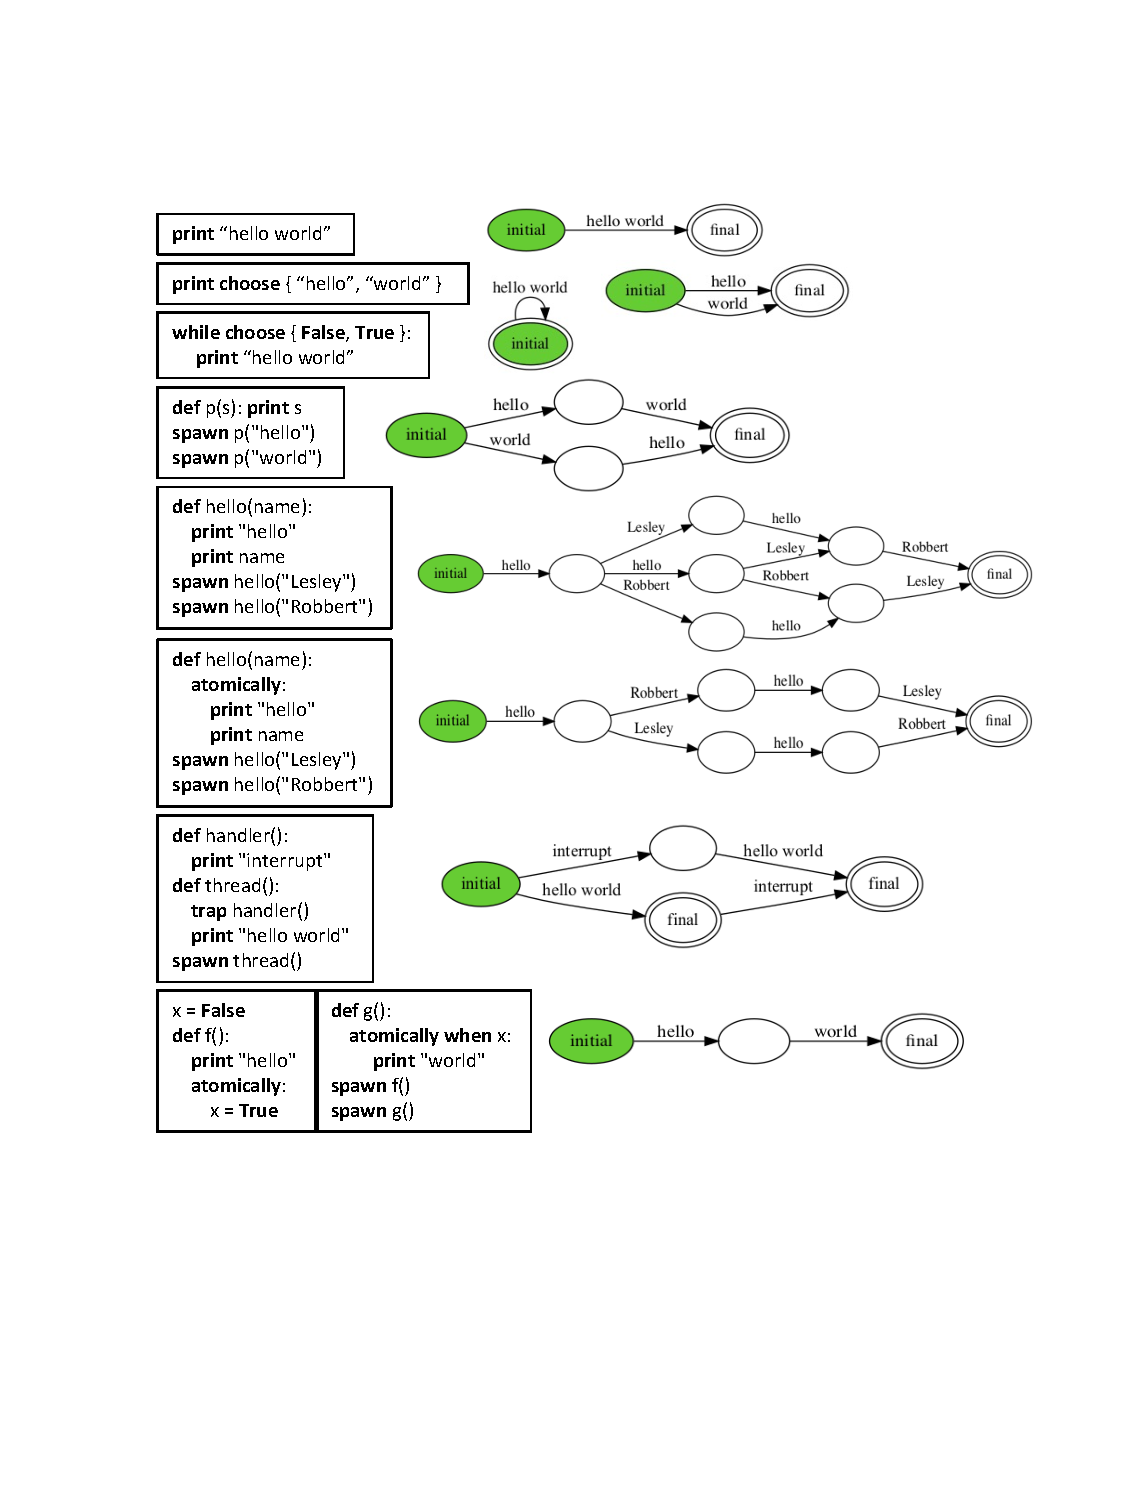
\includegraphics[width=.9\textwidth]{hello.pdf}
\end{center}
\caption{A demonstration of various Harmony language constructs.  The DFAs
are the actual outputs of the given programs.}
\label{fig:helloworld}
\end{figure*}

\section{Introduction}

\emph{Harmony} is a Python-like programming language designed to teach
systems specification, implementation, and verification techniques to
students who do not have a background in formal methods.
Harmony programs, which can be multi-threaded
or distributed, are model checked~\cite{CES86}.
Without any special formalism, Harmony can diagnose a large variety
of problems in programs:
\begin{compactitem}
\item ``Silly errors'': accessing non-existent variables,
divide-by-zero, out-of-bounds array access, dereferencing dangling
pointers, trying to multiply two lists with one another,
and many more.
\item Safety violations: Harmony supports both assertions that must hold in a particular location and general invariants.
\item Liveness violations: not reaching a final state, often due to deadlock or an infinite loop.
\item Faulty behaviors: implementation has behaviors not seen in the specification, such as violations of linearizability~\cite{HW90}.
\item Incomplete behaviors: specification has behaviors not seen with implementation, such as multiple readers not able to get a reader/writer lock simultaneously.
\item Data races: shared variables accessed without a lock.
\item Busy Waiting: waiting for a condition without blocking.
\item Violations of interrupt safety: a race condition caused by the execution
of an interrupt handler.
\item Memory leaks: memory unintentionally allocated in a final state.
\end{compactitem}

\begin{figure*}
\begin{center}
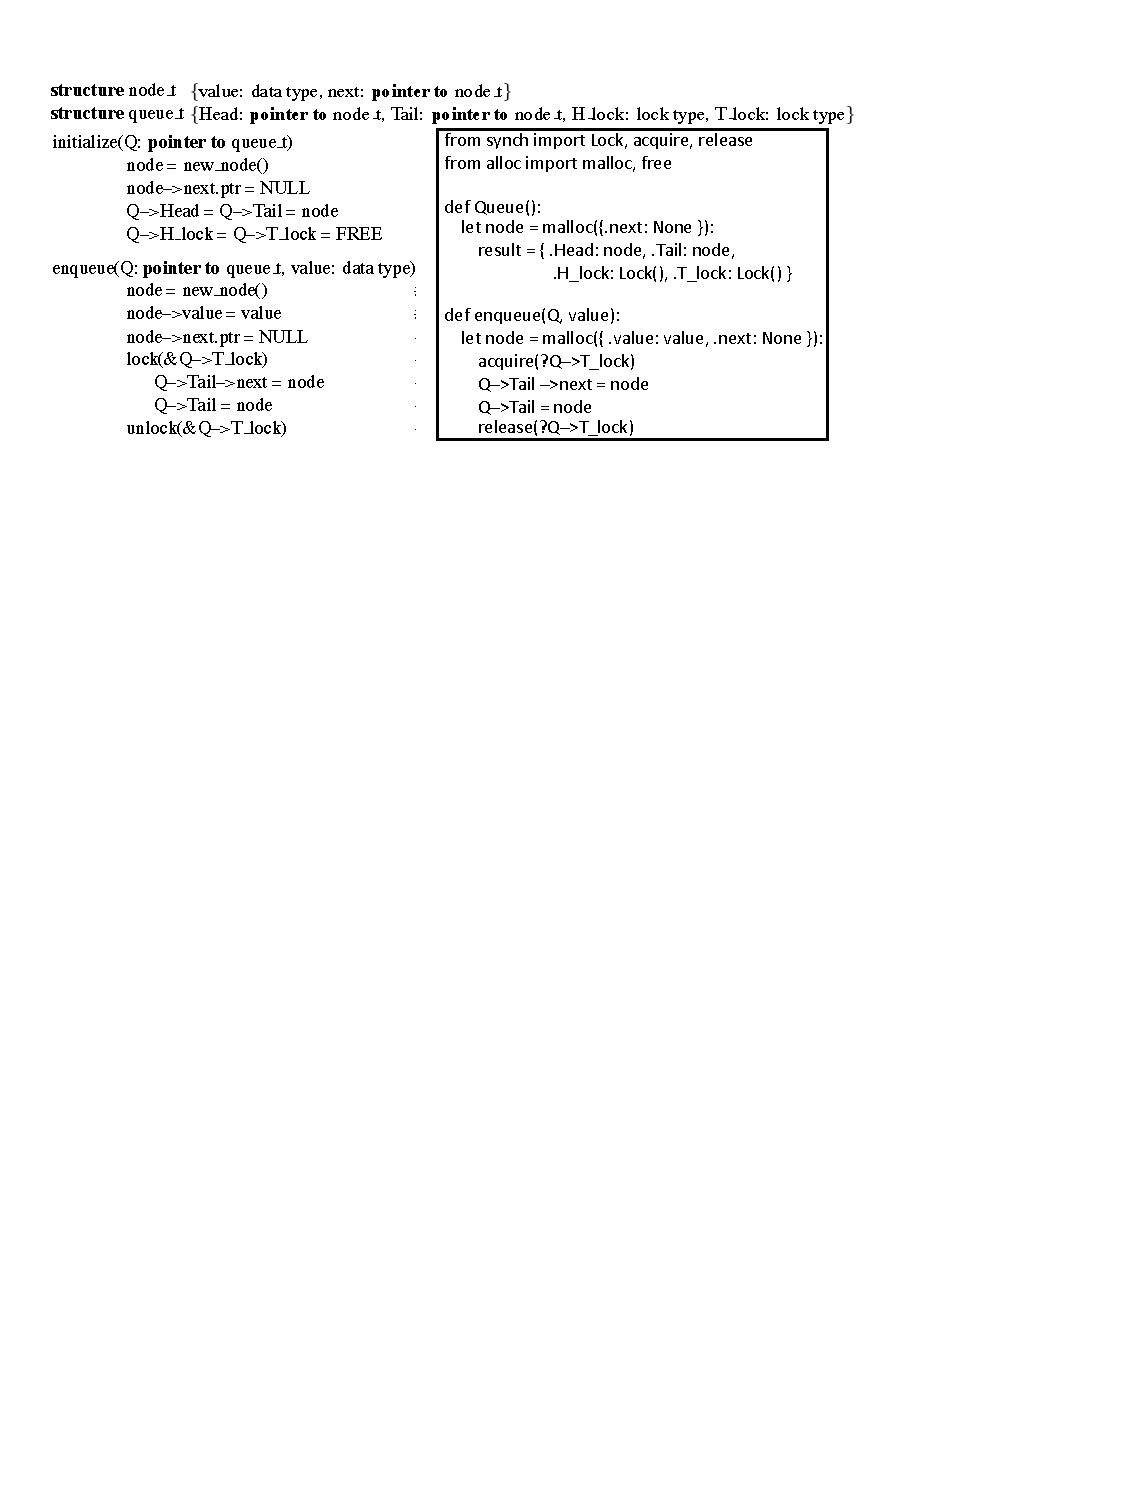
\includegraphics[width=.9\textwidth]{MS.pdf}
\end{center}
\caption{A reproduction of the 1996 Michael\&Scott two-lock concurrent queue
implementation and its equivalent in Harmony (within the box)}
\label{fig:ms}
\end{figure*}

Harmony programs have three sources of non-determinism:
<{choose}> operations that select a value from a set,
\emph{interleaving} due to multi-threading, and \emph{interrupts}.
\autoref{fig:helloworld} demonstrates various non-deterministic
Harmony programs.
Since Harmony programs are model-checked and all possible
executions are explored across a finite set of states, the output of a
Harmony program is a finite automaton that describes all possible
outputs of the program.  Groups of statements can be made atomic
using the <{atomically}> keyword.  Harmony supports
waiting until some condition is reached with its <{when}> statement.

Harmony programs compile to a virtual machine.  The virtual machine
instructions are the units of atomicity.  The Harmony virtual
machine is formally specified using TLA+~\cite{Lamport02}, allowing
Harmony programs to run using TLC, the model checker that comes
with the TLA+ toolbox.  Harmony has its own custom concurrent model
checker that scales significantly better for Harmony programs.

The Harmony language can be used both to \emph{specify} desired
behaviors and to \emph{implement} them.  To check that the implementation
satisfies the specification, the programmer writes a test program that
systematically checks available operations and prints the results.
The test program is first run against the specification, generating
a \emph{behavior automaton}.  The same test program is then run
against the implementation, along with the behavior automaton.
The Harmony model checker generates the Cartesian product of the test program
and the behavior automaton to find discrepancies in the implementation
with respect to its specification.

Harmony supports continuations as first-class objects, allowing the
state of a thread to be saved in a variable and later restored.
Continuations enable the implementation of specialized thread
schedulers as well as the implementation of thread forking by
reinstantiating a saved thread state multiple times.
Other uses include exception handlers, coroutines, and generators.

Harmony has been used to model check the correctness of various lock
implementations, monitors and condition variables (both Hoare and Mesa),
various implementations of concurrent data structures including lock-free
ones, and barrier synchronization implementations.  Harmony has also been
used to model check a variety of distributed algorithms such as two-phase
commit, chain replication, various consensus algorithms such as Paxos,
and the Needham-Schroeder authentication protocols.

Harmony's unique combination of features are
\begin{compactitem}
\item a familiar and easy-to-learn high-level programming language.
\item the ability to concisely specify an interface.
\item the ability to compare behaviors of specification and implementation.
\item the ability to modularly model check programs.
\item support for dynamic memory allocation.
\item support for continuations.
\item support for interrupts.
\item automatic diagnosis of various common problems such as
undesirable busy waiting.
\end{compactitem}

This paper provides an overview of the Harmony language and Charm,
its model checker, and how they may be used by programmers to
specify and implement reliable concurrent and/or distributed systems.

\begin{figure*}[h]
\begin{center}
\begin{tabular}{cc}
{\footnotesize
\begin{tcolorbox}[width=0.45\linewidth]
<{:const:head}>
<{:const:tail}>
<{:const:append}>
<{:const:test_and_set}>
<{:inline:}>
def Lock():
    result = False

def acquire(lk):
    atomically when not !lk:
        !lk = True

def release(lk):
    atomically !lk = False
<{:end:}>
\end{tcolorbox}
}
&
{\footnotesize
\begin{tcolorbox}[width=0.45\linewidth]
<{:inline:}>
def test_and_set(s):
    atomically:
        result = !s
        !s = True

def acquire(lk):
    while test_and_set(lk):
        pass

<{:end:}>
\end{tcolorbox}
}
\\
(a) & (b)
\end{tabular}
\end{center}
\caption{(a) Lock specification and (b) a spinlock implementation based on
a specification of test-and-set}
\label{fig:synch}
\end{figure*}

\section{Harmony Language}

Harmony is heavily based on Python to reduce the learning curve for
users.  Many of Python's powerful constructs and operators are
supported, including sets, lists, tuples, dictionaries, and
comprehensions.  In certain cases Harmony goes further than Python,
for example by allowing sets of dictionaries (Harmony does not have
so-called ``unhashable types'').

Harmony does not
support classes and instead supports memory allocation and pointers
in a way that is familiar to C programmers.  While perhaps this
seems like a step back in language evolution, many synchronization
algorithms in the literature explicitly consider memory accesses,
and this has been a bonus for analyzing such algorithms with Harmony.
Moreover, the Harmony model checker can be used to check for memory
leaks or access to dangling pointers.

For example, \autoref{fig:ms} shows a reproduction of the well-known
Michael\&Scott two-lock concurrent queue~\cite{MS96} along with a
Harmony version of the same algorithm.
Harmony uses the `<{?}>' instead of the `<{&}>' symbol to take the address
of a memory location, but inherits the same <{q->field}> notation
from C to access the given field in the dictionary pointed to by
pointer <{q}>.  <{q->field}> is shorthand for <{(!q)["field"]}> in
Harmony, where `<{!}>' is the Harmony operator to dereference a pointer.
Harmony complains, correctly, about a data race when
there is a concurrent \texttt{enqueue} and \texttt{dequeue} operation
on an empty queue---the implementer should ensure that accesses to the
\texttt{next} field are sequentially consistent.

The Harmony example in \autoref{fig:ms} shows some other language
features in Harmony that are not in Python.
The <{let x = e: S}> statement introduces a new bound variable <{x}>
with value <{e}> that is only valid within the statement block <{S}>.
Harmony does not have \texttt{return}, \texttt{break}, or
\texttt{continue} statements to force the programmer into a purely
nested control flow.  Each method has a variable <{result}> in which
the return value of the method is stored.

A \emph{blocked} thread is waiting on a condition
(for example, a lock becoming available) using the <{when}> statement.
This is implemented in the Harmony virtual machine
by executing in a loop until the condition holds, without changing the
shared state, and thus the thread can only be unblocked by another thread
changing the state.

\emph{Deadlock} is the situation in which threads are waiting for
one another.
In order to make deadlock detection possible, a Harmony program is
required to eventually terminate under fair selection of its
nondetermistic choices.  In other words, from each state there
should always exist an extension of the execution in which the
Harmony program terminates.  Harmony supports \emph{eternal}
threads---threads that never terminate---for example to model
servers.  A Harmony program is considered terminated if it is in a
state in which all its remaining threads are eternal and blocked.

\begin{figure*}[h]
\begin{center}
\begin{tabular}{cc}
{\footnotesize
\begin{tcolorbox}[width=0.45\linewidth]
<{:inline:}>
import list

def Queue():
    result = []

def enqueue(q, v):
    atomically !q = list.append(!q, v)

def dequeue(q):
    atomically:
        if !q == []:
            result = None
        else:
            result = list.head(!q)
            !q = list.tail(!q)



<{:end:}>
\end{tcolorbox}
}
&
{\footnotesize
\begin{tcolorbox}[width=0.48\linewidth]
<{:inline:}>
import queue

const NOPS = 4
q = queue.Queue()

def enq_test(self):
    print("call enqueue", self)
    queue.enqueue(?q, self)
    print("done enqueue", self)

def deq_test(self):
    print("call dequeue", self)
    let v = queue.dequeue(?q):
        print("done dequeue", self, v)

nenq = choose {1..NOPS-1}
for i in {1..nenq}:      spawn enq_test(i)
for i in {1..NOPS-nenq}: spawn deq_test(i)
<{:end:}>
\end{tcolorbox}
}
\\
(a) concurrent <{queue}> module & (b) test program
\end{tabular}
\end{center}
\caption{The (a) specification and (b) test program for a concurrent queue}
\label{fig:queue}
\end{figure*}

\subsection{\texttt{atomically}}

A Harmony program compiles to instructions for a virtual machine.
Those instructions are normally the units of atomicity, but threads
can be temporarily placed in \emph{atomic mode} to prevent instructions
interleaving with those of other threads or interrupt handlers.
At the Harmony language level, even simple statements should not be
assumed to be atomic.
However, statements---including groups of statements---can be tagged with
the \texttt{atomically} keyword to make them execute as if they were
a single atomic instruction.
It is
a \emph{stronger} condition than holding a lock---a lock still allows
concurrent execution of multiple threads, but it prevents multiple
threads from executing in the same critical section.
The <{atomically}> keyword is intended for <{specification}> more than
for <{implementation}> of concurrent algorithms.

For example, \autoref{fig:synch}(a) shows the specification for locks
from the Harmony <{synch}> module that was used in \autoref{fig:ms},
featuring the Harmony <{when}> statement.
\autoref{fig:synch}(b) shows an implementation of the <{acquire}>
method based on a test-and-set primitive, which in turn is
\emph{specified}.
Imprecisely, methods that use the <{atomically}> keyword are specifications.
Important is the notion of modularity that is implied here.
Harmony can model check the implementation of \autoref{fig:ms} using
the specification of a lock in \autoref{fig:synch}(a).
Separately, Harmony can check the correctness of the implementation in
\autoref{fig:synch}(b) against the specification in
\autoref{fig:synch}(a).

The Harmony distribution comes with a collection of specifications,
each often with multiple implementations.  The lock specification
comes with the spinlock implementation of \autoref{fig:synch}(a), but
also a ticket lock implementation and one based on continuations and
a queue of blocked threads.  The distribution also includes various concurrent
queue implementations, including the lock-free implementation
of~\cite{MS96}.

\subsection{Checking an implementation}

The Harmony language allows objects such as locks and concurrent queues
to be specified and implemented in separate programs.  But the programs
are not \emph{active} as they are just a collection of method definitions.
A model checker can only check behaviors, but these programs have empty
behaviors.
Suppose we want to check the correctness of the concurrent queue
implementation of \autoref{fig:ms}.  First, we would need a specification
of a concurrent queue.  Second, we would need a test program that tries
various concurrent interleavings of <{enqueue}> and <{dequeue}> operations.

\autoref{fig:queue}(a) shows the specification of a concurrent
<{queue}> module.  A queue is represented as a list.
The <{enqueue}> method appends a value onto the end of the list,
while the <{dequeue}> method extracts the head, both as atomic actions.

To test a concurrent queue, we need to perform a set of <{enqueue}>
and <{dequeue}> operations concurrently.  \autoref{fig:queue}(b)
shows how this can be specified in Harmony.  The test program spawns
<{NOPS = 4}> threads, at least one of which does an <{enqueue}>
operation and at least one of which does a <{dequeue}> operation.
A thread that does an <{enqueue}> enqueues its identifier <{self}>.
The program includes a <{print}> statement at the beginning and end
of every queue operation.  Think of the <{print}> statements as
\emph{annotations} that tell Harmony what the interesting events
are with respect to queue operations.  We will use the output of
those <{print}> statements to compare the behavior of an implementation
with that of its specification.

\begin{figure*}
\begin{center}
\begin{tabular}{l|c|c|c|c}
           & <{NOPS=2}> & <{NOPS=3}> & <{NOPS=4}> & <{NOPS=5}> \\ \hline\hline
queue specification    &  30/0.0 &  350/0.0 &  3,385/0.0 &    32,010/0.1 \\ \hline
queue impl. w/o check  &  90/0.0 & 1905/0.0 & 39,519/0.1 & 1,089,222/5.6 \\ \hline
queue impl. with check & 101/0.0 & 2566/0.0 & 75,974/0.3 & 3,400,555/22.8 \\
\end{tabular}
\end{center}
\caption{The number of states generated by the model checker and the
model checking time (in seconds) for running \autoref{fig:queue}(b).
This is done for three configurations, varying the value of <{NOPS}>:
the specification (\autoref{fig:queue}(a)), a simple linked list
implementation using locks, and the same implementation combined with
the behavior automaton generated by the first configuration.  The
hardware consisted of a 2.8 GHz Quad-Core Intel Core i7
(2 hyperthreads per core) with 2,133 MHz LPDDR3 memory.}
\label{fig:qcmp}
\end{figure*}

The test program is similar to what a programmer might have written
as a unit test.  The programmer would run the program a bunch of
times and look at the output in order to see if it looks reasonable.
Doing so is difficult and error prone, as the output tends to be
complex and---in the mess of many lines of output---it is easy to
overlook problems such as two threads dequeuing the same item or
items being dequeued in the wrong order.  Not only that, but the
programmer would need to run this test program many times and check
the output each time.  It is hard to write a program that checks
the output automatically as it is difficult to characterize what
correct outputs are.

This process is automated in Harmony.  The approach is to
run the model checker twice.  The first time, the test program is
run against the specification of the concurrent queue.  Harmony
outputs a DFA such as shown in \autoref{fig:helloworld}.  The second
time, the same test program is run against the implementation of the
concurrent queue, but with the inclusion of the DFA.  The model
checker ends up executing the Cartesian product of the implementation
and the DFA and ensures that every behavior of the implementation
program (in terms of its print statements) is also a behavior of
the specification program.  In case the implementation has a behavior
that is not allowed by the specification, the model checker can
provide the shortest counter-example.

\autoref{fig:qcmp} shows measurements taken from running
Harmony against the test program in \autoref{fig:queue}(b).
The Harmony compiler allows both constants and modules to be
specified on the command line, so the test program can easily be
run with different versions of the <{queue}> module and different
values for <{NOPS}>, the number of threads spawned to
perform a queue operation.  The table has a row for three different
configurations and a column for four different values for <{NOPS}>.
It is clear that running the test program against the specification
involves significantly fewer states, and therefore less time, than
running the test program against an implementation, particularly
if the behavior of that implementation must be checked as well.

In practice, <{NOPS = 4}> is probably sufficient to check the
correctness of a concurrent queue implementation.  Note, however,
that if there are more than two operations to check, the model
checking time will also increase.  In such cases, it usually suffices
to run all pairs of read-only and read-write operations.

Modularity allows larger systems to be model checked in a way
that would not be tractable otherwise.
With Harmony, one can check the implementation of a lock separately,
but use the specification of the lock in the implementation of the
queue.  Similarly, one can check the implementation of a queue,
but then use the specification of the queue in a larger application.
Doing so is essentially a form of
\emph{Partial Order Reduction}~\cite{Owicki75,Lipton75,Val91},
replacing the <{enqueue}> and <{dequeue}> implementations
by atomic actions.

\begin{figure}
\begin{center}
{\footnotesize
\begin{code}
<{:inline:}>
import list

def Lock(held):
    result = { .held: False, .blocked: [] }

def acquire(lk):
    atomically:
        if lk->held:
            stop lk->blocked[len lk->blocked]
        else:
            lk->held = True

def release(lk):
    atomically:
        if lk->blocked == []:
            lk->held = False
        else:
            go (list.head(lk->blocked)) ()
            lk->blocked = list.tail(lk->blocked)
<{:end:}>
\end{code}
}
\end{center}
\caption{FIFO lock using continuations}
\label{fig:continuation}
\end{figure}

\subsection{Continuations}

The Harmony <{stop x}> expression stops the current thread and saves
its state in the variable <{x}>.  Another thread can resume the
thread using the statement <{go x r}>, which causes the original
thread to resume, with the <{stop x}> expression evaluating to the
value <{r}>.  \autoref{fig:continuation} shows another implementation
of the lock specification of \autoref{fig:synch}(a) using continuations,
where blocked threads are placed on a FIFO queue and released in
that order.  Besides synchronization and scheduling, continuations
also enable the implementation of a primitive such as Posix
\texttt{fork}.

\subsection{Interrupts}

Correct interrupt handling is another difficult aspect of
systems programming.  Interrupt handlers typically have various
stringent limitations in what they are allowed to do in order
to ensure the absence of race conditions due to re-entrant code.
The Harmony <{trap f(x)}> statement sets an interrupt handler
<{f(x)}> to be called at an unspecified later time.  You can think
of it as setting an unspecified timer, but it can model any type
of interrupt.  In addition, the Harmony <{setintlevel L}> statement
enables or disables interrupts and returns the old interrupt level.
The model checker tries calling the interrupt handler at every
possible point in the execution of the Harmony program.

\begin{figure}
\begin{tabular}{|l|l|}
\hline
Boolean & <{False}>, <{True}> \\
\hline
Integer & <{..., -2, -1, 0, 1, 2, ...}> \\
\hline
String & <{"example"}>, <{.example}> \\
\hline
PC & (program counters) \\
\hline
Dictionary & <{{ .acct: 12345, .valid: False }}> \\
\hline
Set & <{{}, { 1, 2, 3 }, { False, .id, 3 }}> \\
\hline
Address & <{?lock, ?flags[2], None}> \\
\hline
Context & (generated by <{stop}> expression) \\
\hline
\end{tabular}
\caption{Harmony values}
\label{fig:values}
\end{figure}

\subsection{Distributed Programming}

Harmony can be used to model a distributed system in which the
only shared variable is a set of messages representing the network.
From a model checking perspective, it is convenient that message and
timer handling can be performed atomically, as the only interaction
between threads is through the network variable.
A message is sent by atomically adding a message to the network:
<{def send(m): atomically network |= {m}}> (`<{|}>' is the symbol for
the union operator in Python).
To receive a message, a program can use the Harmony <{when}>
statement to wait for a message.  Typically, however, the program
does not want to receive just any message, but a message that satisfies
certain conditions such as: \emph{wait for the next message that is addressed
to me and has a sequence number larger than 3}.
For this, Harmony supports the <{exists}> clause and allows
<{when}> clauses to be nested:
<{atomically when exists m in network when (m.dst == self) and (m.seq > 3): ...}>
With these constructs, Harmony can be effectively used as a
model checker for distributed algorithms.

\section{Harmony Virtual Machine}

The Harmony Virtual Machine (HVM) is fully specified in approximately
1000 lines of TLA+.
Below we summarize its most important aspects.

\subsection{Values}

Harmony has 8 types of values listed in \autoref{fig:values}.
There are no exceptions: a set can contain dictionaries, a dictionary
can map dictionaries to dictionaries, and so on.  Unlike many
object-oriented programming languages including Python, the programmer never
has to specify what it means for two values to be the same or what the
hash of a value is.

Any two values can be compared using the standard comparison operators.
If two values have different types, then their order is defined as by
the order in \autoref{fig:values} (e.g., <{False < 0}>).
For any two values of the same type, Harmony defines a deterministic order.
For example, for two sets, the sets are first converted into ordered lists
and then lexicographically compared, so that <{{ 1, 2 } < { 1, 3 }}>.
(Note that, unlike Python, the $<$ operator is a total order and
$<$ on sets does not represent the subset relationship.)
Dictionaries are lexicographically ordered by their (key, value) pairs.

The strings <{"example"}> and <{.example}> are the same---the latter
form is convenient for use in dictionaries.
An \emph{address} represents a path in a hierarchy of dictionaries, with
<{None}> being the empty path.
Examples of \emph{program counters} include method constants and program labels.
A \emph{context} represents the state of a thread.  It includes a program
counter, a map of local variable names to values, and a stack of values.
% Harmony makes no difference between lists and tuples and implements
% both as dictionaries from integers to values.
% So <{[7, 4] = (7, 4) = { 0: 7, 1: 4 }}>.
% Note that <{[7, 4][0] = 7}>, as expected.
% The empty dictionary is represented as either <{()}> or <{[]}>
% (<{{}}> is the empty set).

Except for <{choose}>, any operation on values is a deterministic
function and unequivocally defined in the formal specification of the
Harmony virtual machine.
For example, like Python, Harmony supports merging of dictionaries
using the union operator, but, unlike Python, Harmony defines
what happens when two dictionaries have the same key but different values.
In that case, Harmony will use the maximum value according to the order
defined above.
For dictionary  intersection, Harmony uses the minimum value instead.
Doing so makes dictionary union and intersection deterministic and
commutative.  Moreover, Harmony represents multisets as dictionaries
of values to multiplicities.  Using Harmony's rules on dictionary union
and intersection, union and intersection on multisets are correctly
defined.

\subsection{State}

The state of the HVM consists of three variables:
\begin{compactitem}
\item a dictionary of shared variable names to values;
\item a bag (multiset) of contexts, one for each thread;
\item a set of \emph{active} contexts.
\end{compactitem}

Harmony uses a multibag to keep track of the states of the threads
because threads can be in the same state.
Threads do not have unique identifiers, reducing combinatorial
state explosion in the model checker.

A context is active if it can make a transition.
Contexts can be atomic or not---the HVM prevents multiple atomic
contexts from being atomic simultaneously.  Therefore, the active set
either contains a single atomic context or it contains all contexts
in the domain of the context bag.

The initial state consists of an empty dictionary of shared variables and
a single atomic context with program
counter 0 in both the context bag and the active set.

Harmony also allows the user to specify a determistic finite automaton
(DFA) to check the legality of the output of the program to be
checked.  In that case, the state of the automaton is also made
part of the HVM state, so that the HVM maintains the product of the
program state and the DFA state.

\subsection{Transitions}

The HVM makes a transition by executing an HVM instruction using
one of the contexts in the active set.  There are about 30 basic
transitions, which, for this paper, we classify as follows:

\begin{compactitem}
\item \emph{basic operations}: a deterministic operation that only
involves a single context and no shared state, such as pushing a value
onto the stack or increment the program counter.
\item \texttt{Frame/Return}: method start/end.
\item \texttt{Choose}: nondetermistic selection from a set.
\item \texttt{Apply}: method call \emph{or} index into a dictionary.
\item \texttt{Spawn}: thread creation.
\item \texttt{AtomicInc/AtomicDec}: atomic section enter/leave.
\item \texttt{SetIntLevel}: interrupt enable/disable.
\item \texttt{Stop/Go}: continuation save/restart.
\item \texttt{Assert}: value check.
\item \texttt{Print}: output.
\end{compactitem}

Each transition modifies at least the context bag and set of active
contexts.
A few operations (\texttt{Store}, \texttt{Stop}, and \texttt{Del})
also modify one of the shared variables.
Below we describe in more detail some of the more unusual ones.

\paragraph{Choose.} \texttt{Choose} pops a set value of the stack
and pushes a selected element back onto the stack.  The model checker
tries each selection.

\paragraph{Apply.}  \texttt{Apply} pops two values $f$ and $x$ of the stack,
\emph{applies} $x$ to $f$, and pushes the resulting value back onto the
stack.  What \emph{applies} means depends on the type of $f$.  If $f$ is
a PC value, then it means invoking method $f$: it pushes the return address
and $x$ onto the stack and sets the program counter to $f$.  If $f$ is a
dictionary, then it means pushing the value corresponding to key $x$ onto
the stack.  This way, a dictionary acts much like a method that maps keys
to values.  If $f$ is a string, then the operation returns the $x^{th}$
character of the string.

\begin{comment}
\paragraph{Frame/Return.}  \texttt{Frame} is the first operation of
a method and \texttt{Return} its last.  \texttt{Frame} pops a value of
the stack and assigns it to the argument (or argument list) of the
method.  It also saves the local variables onto the stack and sets the
value of the <{result}> variable to <{None}>.  The operation of
\texttt{Return} depends on whether the stack is empty of not.  If empty,
\texttt{Return} terminates the thread by removing the context from the
context bag and replacing the active set with the domain of the context bag.
If the stack is not empty, then (1) the saved local variables are popped
and restored, (2) the return address is popped and assigned to the
program counter, and (3) the value of <{result}> is pushed onto the
stack.
\end{comment}

\paragraph{Spawn.}  Spawn pops a program counter and argument from the
stack and uses them to create a new context.  The new context is added
to the context bag.  Also, if the current context is not atomic, then
the new context is also added to the active set.

\paragraph{AtomicInc/AtomicDec.}  A context contains a counter that,
if non-zero, puts the context in atomic mode.
<{atomically}> statements can be nested: at the beginning, the
counter is incremented; at the end, it is decremented.
When incremented from 0 to 1, the operation replaces the active
set of context with just the current context.  When decremented
from 1 to 0, the active set is replaced with the union of the
new context and the domain of the context bag.

\begin{comment}
\paragraph{SetIntLevel.}  A context contains a boolean that determines
if interrupts are enabled or not.  \texttt{SetIntLevel} pops the
new interrupt level and pushes the old.  Supporting interrupts is
important.  First, writing multi-threaded programs that also need
to handle interrupts is difficult.  Second, distributed algorithms
often require timer interrupts to trigger actions such as retransmissions.
\end{comment}

\paragraph{Stop/Go.} \texttt{Stop} saves the current context
(with its program counter incremented) in a specified shared location
(such as the tail of a scheduling queue) and removes the context
from the context bag and active set.  If the context was atomic
(which is usually the case), the active set is replaced with the
domain of the context bag.  Even though its atomic counter is not
zero, the stopped context is not considered atomic at this time,
but will resume being atomic once it is scheduled to run.

\texttt{Go} pops a context value and a return value of the stack,
pushes the return value onto the stack of the popped context, and adds
the context to the context bag.  If the current context is not atomic,
then the restored context is also added to the active set.
A stopped context can be re-instantiated multiple times, allowing
programmers to implement thread forking.

\paragraph{Assert.}  \texttt{Assert} pops a boolean value and increments
the program counter.  If the value is <{False}>, the HVM aborts.

\paragraph{Print.}  \texttt{Print} pops a value of the stack and increments
the program counter.  In case a behavior automaton has been specified, the
value is applied to the DFA state and checked for validity.
To reduce state explosion, the HVM does not keep track of the value itself
in the state (like keeping the value in a shared list as part of the state).
Instead, Harmony keeps printed values on the edges between the states.

\subsection{Model Checker}

\emph{Charm}, Harmony's concurrent model checker, is an explicit state model
checker that computes a \emph{Kripke structure}~\cite{Kripke1963}
(essentially, a graph) of states reachable
from the initial state in a breadth-first manner, stopping only if
it encounters an error (such as divide-by-zero or a failing assertion)
or until there are no more new states.

There are three sources of nondetermism in Harmony: \texttt{Choose}
operations, thread interleaving, and interrupts.
When it comes to interleaving, an important observation is that
local operations on the state of a context (updates to its program
counter, local variables, or stack) are not visible to other threads.
An important optimization that significantly
reduces the size of the set of generated states is to treat a
sequence of operations as atomic if only its first operation is an
operation that accesses the shared state (\texttt{Load}, \texttt{Store},
\texttt{Del}, or \texttt{Stop}) or a \texttt{Choose} or \texttt{Print}
operation.  We call such operations \emph{breakable}.
Note that this optimization is essentially Partial Order
Reduction~\cite{Val91}.

Reducing the state space this way is highly effective for Harmony.
For example, when model checking Peterson's algorithm expressed in
Harmony, the number of states is reduced from 7927 to 104 states.
In the case of the Knuth-Yao algorithm (which is not concurrent but
involves choices), the number of states is reduced from 258 states
to 14.

Given a state and a context, Charm starts with applying the instruction
pointed to by the context's program counter to the state.
Then it continues to apply instructions as long as
the active set is the singleton set (such as when the thread is in
atomic mode) or, if not, as long as the next instruction is not
breakable.  Only the resulting state is added to the Kripke structure,
and the edge indicates the starting context.  During this loop, Charm
does check if the same state recurs---if so, it aborts
and reports an infinite loop.

In the case the first instruction is a \texttt{Choose} instruction,
Charm will try all possible choices for the set value
on top of the stack.  If not, Charm will check to
see if a trap is outstanding and interrupts are enabled.  If so,
Charm will try an interrupt transition as well.

In practice, about half of the work of the model checking is trivially
parallelizable, allowing for significant speedups on multi-core machines.

\subsection{Data Race Detection}

A data race occurs when two or more threads simultaneously try to
access the same shared data location, at least one of which is a
\texttt{Store}, \texttt{Stop}, or \texttt{Del} instruction.  Data races
can also occur in a single thread that experiences an interrupt.  Harmony
only considers this a problem it at least one of those threads is
not in atomic mode.  After all, we do not want to consider accesses
to a spinlock as a problem.  Also, the Harmony language allows
shared variables to be tagged as \emph{sequentially consistent},
effectively turning off data race detection.  Charm maintains on
each edge of the Kripke structure a list of accesses that were made
during the transition.  After all transitions from a state have been
computed, Charm checks for data races.

\section{Harmony Compiler}

The compiler translates the Harmony language to a sequence of HVM
instructions.  The compiler is mostly straightforward.  This section
describes some of its unusual features.

To help the programmer reason about the behavior of the generated code,
the compiler preserves the left-to-right evaluation order of
expresssions.  In other words, if expression $e_1$ appears before
$e_2$ in the source language, then $e_1$ is evaluated before $e_2$
in the HVM translation.  There is one exception, for the Harmony/Python
$e_1~<{if}>~c~<{else}>~e_2$ expression, $c$ is evaluated first, and
depending on the outcome, either $e_1$ or $e_2$ is evaluated.

The compiler performs some standard optimizations that do not re-order
expression evaluations, such as constant folding and jump threading.
An unusual optimization is \emph{dead variable elimination}:
local variables that are no longer in use are automatically removed
from the state using the HVM \texttt{DelVar} instruction.  The reason
for this is to reduce state explosion by removing state that is no
longer in use.

\section{Analysis}

After running the Charm model checker, there are two cases to
consider.  If Charm aborted due to some problematic transition,
then Charm reports the shortest path as a so-called \emph{counter-example}.
If not, the resulting graph is analyzed for various other problems,
including deadlock, busy waiting, and executions
that ended in a state that is not considered final according to the
behavior DFA if specified.  We detail below how these problems are
found.

\paragraph{Deadlock and Faulty Behavior.}

Harmony transforms the Kripke structure into a DAG of its strongly
connected components.  The states in the sink components of this
DAG can be considered the terminal states of the Harmony program.
States in which the context bag is empty represent states in which
all threads have terminated.  In the case the context bag is not
empty, we check if there are any non-\emph{eternal} contexts or
contexts that are not blocked.
If so, Harmony reports a \emph{deadlock}. If there
is no deadlock and a behavior automaton was specified, Harmony also
checks if the automaton is in a terminal state.  If not, a
\emph{behavior violation} is reported.

\paragraph{Active Busy Waiting.}

As mentioned above, a thread is considered blocked if it can only
modify the shared state if another thread updates the shared state
first.  This is not usually a problem: a thread waiting on a lock
in a spinloop is a common way of synchronizing threads, and Harmony
does not report such issues.  We call this \emph{passive busy
waiting} as the thread does not modify the state.

A thread is considered \emph{actively busy waiting} if it is in a
loop updating the shared state, but cannot
escape its strongly connected component without another thread
also updating the shared state.  A common example of this is a
synchronization algorithm that checks for a condition in a loop,
acquiring and releasing the lock each time.  Harmony checks each
strongly connected component for the existence of such situations
and reports the shortest example.

\paragraph{Incomplete Behavior.}

The Kripke structure can be considered as a non-deterministic
automaton, with on each edge zero or more \emph{symbols} (values
that were printed).  If a behavior automaton was specified,
then there are now two automata: the specified automaton
${\mathcal S}$ that was presented to Charm as an input as
part of the \emph{specification}, and the generated automaton
${\mathcal I}$ that was generated by the given Harmony
\emph{implementation}.  Harmony already checks on-the-fly whether
${\mathcal I} \subseteq {\mathcal S}$, that is, that every
behavior (sequence of symbols) of the implementation is also a
behavior of the specification.  Harmony also checks if
${\mathcal S} \subset {\mathcal I}$ and, if so,
produces a warning.
Although not currently performed automatically, it is possible to compute
${\mathcal S}~\backslash~{\mathcal I}$
to generate an automaton for all behaviors allowed by the
specification that are not in the implementation.

Having such behaviors is not always a problem, but it can be.  For
example, a reader/writer lock implemented as a plain lock meets the
specification of a reader/writer lock, but it does not allow multiple
readers in the critical section.  Unfortunately, checking ${\mathcal
S} \subset {\mathcal I}$ does not scale well in general and can
only be done for relatively small Kripke structures.

\paragraph{Constructing a Counter-Example.}

When Charm finds a problematic state or transition, it outputs
a detailed trace that is called a \emph{counter-example}.
Harmony always outputs the shortest such trace.
For ease of debugging, traces are ordered first by the number of
context switches they make, and then by the number of states on
the path.
However, in order to save memory, Charm does not actually keep
the required information during the construction of the Kripke
structure.  In particular, its edges only contain the context,
whether an interrupt occurred, and the choice if any.
Thus, in order to reconstruct the
counter-example, Charm runs the HVM one more time, this time
re-evaluating the edges along the path and outputting the
detailed information about each transition.

\begin{figure}
\begin{center}
{\footnotesize
\begin{code}
<{:inline:}>
from synch import Lock, acquire, release

const N = 5
forks = [Lock(),] * N

def diner(which):
    let left, right = (which, (which + 1) % N):
        while choose({ False, True }):
            acquire(?forks[left])
            acquire(?forks[right])
            # dine
            release(?forks[left])
            release(?forks[right])

for i in {0..N-1}: spawn diner(i)
<{:end:}>
\end{code}
}
\end{center}
\caption{Dining Philosophers in Harmony}
\label{fig:diners}
\end{figure}

\begin{figure*}
\begin{center}
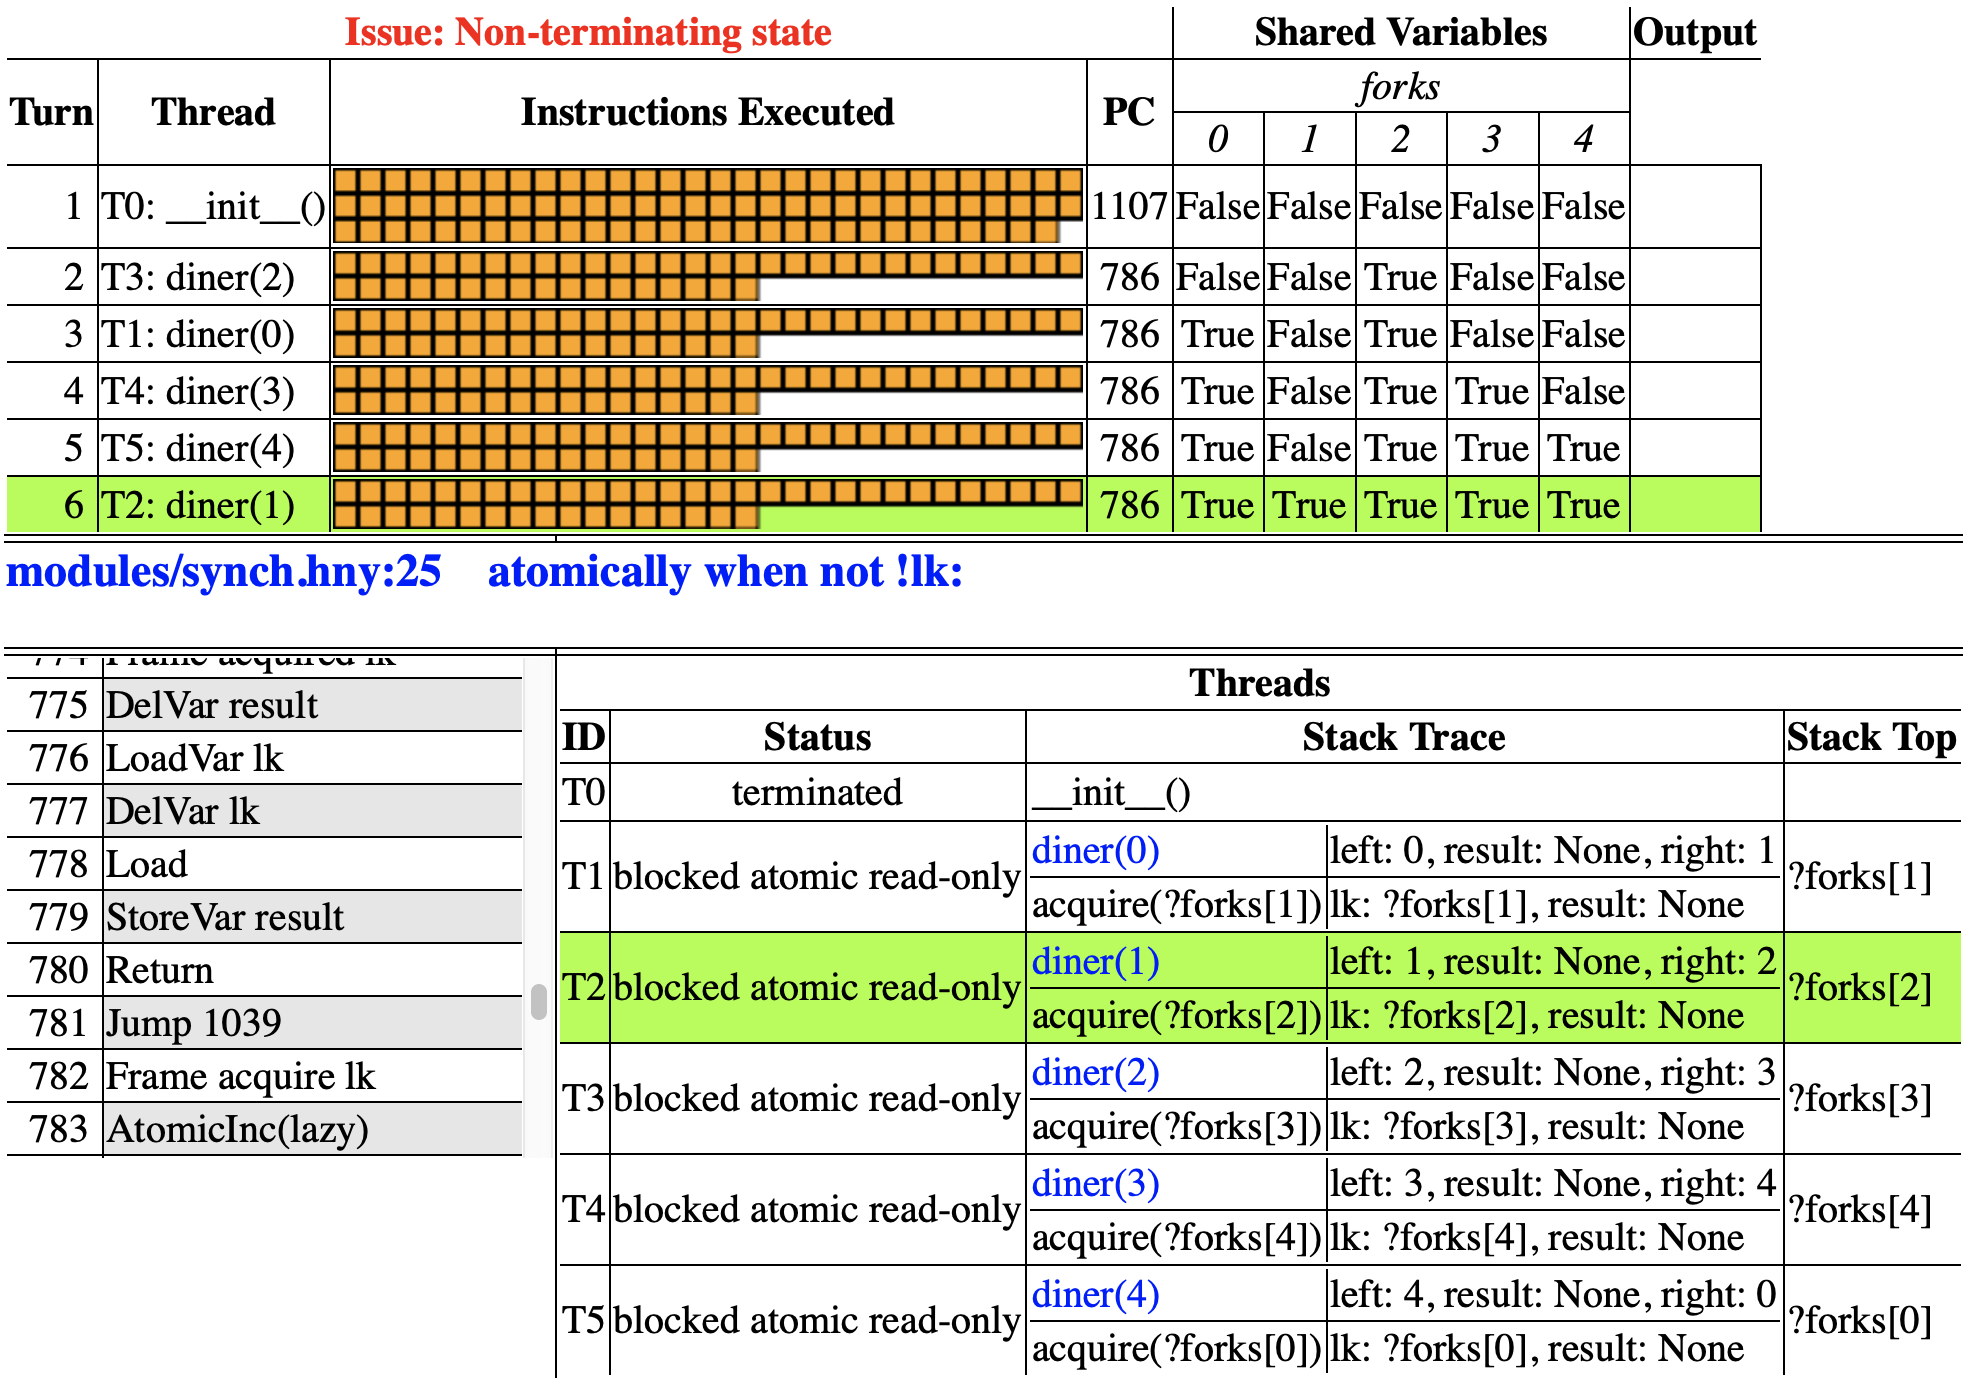
\includegraphics[width=\textwidth]{diners.png}
\end{center}
\caption{The HTML output of running the Dining Philosophers program}
\label{fig:dinersHTML}
\end{figure*}

\section{Debugging}

If Charm determines a problem, it outputs the shortest counter-example that
it could find.  However, this counter-example is at the level of the HVM,
not the Harmony program that the programmer wrote.  Without help it can be
difficult to dig through a list of HVM instructions.
Harmony includes tools to quickly focus on the root cause of the
problem without having to look at the HVM instructions themselves.
In particular, in case of a problem, Harmony outputs a compact
but detailed and interactive overview of the problem in HTML format that
can be accessed from any web browser.

For example, \autoref{fig:diners} shows the implementation
in Harmony of the famous Dining Philosophers problem, where 5 philosphers
share 5 forks (represented by 5 locks).
The philosophers end up being deadlocked
if they all pick up their left fork before any philosopher picks up
their right fork.
Harmony quickly finds the problem and produces the output
shown in \autoref{fig:dinersHTML}.

The little orange boxes represent individual HVM instructions of
the problematic trace.  The programmer can click on any such box
to see the state at that time and the HVM instruction it is executing,
or can navigate in various ways (forwards one step, backwards
one step, jump to the next line of Harmony code, or jumps forwards
or backwards to a context switch between threads).  The actual HVM
code is in the lower left of the output.

However, users first want to focus on the rows in the top table.
In this particular example, there are 6 threads, the thread that
first runs and the five threads that are spawned by it.  They take
``turns'' by context switching.  In this particular trace, <{diner(2)}>
runs first and acquires <{forks[2]}>, its left fork.  In the table
in the lower-right, you can see that the thread is currently blocked
and in atomic as well as read-only mode (because conditions in a <{when}>
clause are not allowed to modify state).  You can also see its stack
trace: it is trying to acquire <{forks[3]}>, its right fork (executing
the code in \autoref{fig:synch}(a)).  Next <{diner(0)}>, <{diner(3)}>,
<{diner(4)}>, and <{diner(1)}> take similar turns.  All threads end up
blocked waiting for another thread to release a lock---a classic
deadlock situation.

Should the programmer need more detailed information, then they can
run through the counter-example step-by-step, forwards and backwards,
as explained above.

\section{Limitations}

While Harmony has proven itself to be effective and even fun to use
for a large variety of synchronization problems and distributed
algorithms, it is not a panacea.  At the core of Harmony is a model
checker and---even with all its optimizations---it can still suffer
from combinatorial state explosion in programs that have too many
threads or too many non-deterministic choices.  Nonetheless, because
of its systematic state exploration, many problems can often be
uncovered in small scenarios with few threads and few choices.
Harmony's support for anonymous threads is useful for scaling when
there are many similar threads that do not need to know their own
identifier.  Also, Harmony's support for modular model checking
allows implementing larger systems using the specifications of smaller ones.

Currently there is no compiler that generates production code from
a Harmony program.
Because it is close to languages such as Python and C, it tends to be fairly
easy to hand-translate code developed in Harmony to a desired target
programming language.  However, such hand-translation could easily
introduce a bug that did not exist in the Harmony code.
A Harmony compiler would have to be able to recognize constructs such as
the test-and-set specification in \autoref{fig:synch}(b) and generate
a hardware test-and-set instruction.

Finally, the Harmony language currently does not have a formal definition
itself, and there is no guarantee that the compiler itself is correct.
Harmony compiles to a virtual machine code that is fully formally
specified in TLA+, and this is the level of abstraction where model
checking occurs.

\section{Related Work}

Harmony is preceded by many other model checkers and accompanying
languages.  This section mentions some of Harmony's strongest influences.

PlusCal~\cite{Lamport09} is an imperative programming language that,
after translation to TLA+~\cite{Lamport02} (a formal verification
language), can be run through the TLC model checker.  Harmony also
supports compilation to TLA+.  While similar in spirit to Harmony,
Harmony first compiles to a virtual machine that is close to CPUs
like x86, ARM, and RISC-V, using a stack and common control flow
techniques.  The resulting HVM has a TLA+ specification.  PlusCal,
instead, \emph{trans\-piles} to TLA+ (source-to-source translation).
Informally, the gap between PlusCal programs and their TLA+
representations is much smaller than the gap between Harmony programs
and their TLA+ representations, making PlusCal programs more amenable
to formal verification.  On the other hand, working effectively
with PlusCal does require significant knowledge of TLA+, increasing
the learning curve.

Promela~\cite{SPIN} is a programming language that serves as input
to the SPIN model checker.  Promela has many of the same features
as Harmony and also includes behavior checking.  Promela
does not have a call stack and does not support procedure calls,
making it hard to do modular development and verification.

Zing~\cite{Zing} is a modeling language that, like Harmony, compiles to an
intermediate language that resembles a conventional processor,
including a call stack and dynamically allocated memory.  Like
Harmony it supports procedure calls and concurrency.  Zing goes
further in that it also support object-orientation.  Zing is
mostly used as an intermediate language, transpiled from sources
written in languages such as C\#.

Java Pathfinder~\cite{Pathfinder} and JBMC~\cite{JBMC} are model
checkers for Java bytecode, and,
like Charm, can diagnose data races and deadlock in concurrent
programs.  Because they operate at the level of Java bytecode, they
have no support for atomic code blocks, which allows Harmony to be
used both as a specification and an implementation language.
Particularly the Harmony <{atomically when}> statement is very
useful as a specification construct, for example to specify new
synchronization primitives.

DSLabs~\cite{MWA19} is an educational framework for model checking distributed
systems.  Distributed algorithms are specified in Java in terms of
nodes, messages, and timers in an event-driven style.  DSLabs does not
support model checking sequential or concurrent programs.  Java
also has the disadvantage that it is a verbose language.  Just the
boilerplate for the Paxos project in DSLabs is well over 100 lines
of Java code.  The entire Paxos implementation in Harmony is less
than 50 lines.

Dist\-Algo~\cite{DistAlgo} is a programming language based on Python to
simplify the specification and verification of distributed algorithms.
Dist\-Algo includes a framework for runtime checking of safety and liveness
properties~\cite{LS20}.

\bibliographystyle{alpha}
\bibliography{paper}

\end{document}
